\documentclass[a4paper]{article}

\usepackage{amsmath}
\usepackage{amssymb}
\usepackage{amsfonts}
\usepackage{amsbsy}
\usepackage[catalan]{babel} % Language 
\usepackage{fontspec}
\usepackage[margin=2cm]{geometry}
\usepackage{graphicx}

\setlength{\parindent}{0pt}
\setlength{\parskip}{1em}

\newcommand{\verteq}{\rotatebox{90}{$\,=$}}
\title{Tema 2: Visualització de dades}
\author{Joan Marcè Igual}

\begin{document}
\maketitle

\section{Introducció}

Antigament les dades eren molt fàcils, l'estadístic mateix podia anar a qualsevol lloc i mesurar el que li interessés. Avui en dia amb el \emph{Big Data} això és força diferent. Tot i així en tots dos casos les dades solen tenir més de dues dimensions. 

\emph{Fischer} (estadístic famós) fa un temps va recollir una sèrie de dades sobre peixos, va obtenir 4 tipus de dades diferents cosa que feia difícil la visualització simultània d'aquestes dades.

\section{Anàlisi de Components Principals (PCA)}

\textbf{Objectiu}: reduir la dimensió preservant la major part de la informació \emph{rellevant} (variància). 

\textbf{Exemple}: es vol projectar un llapis (objecte en 3D) en un pla (2D) (Figura~\ref{fig:llapis}).

\begin{figure}[h!]
	\centering
	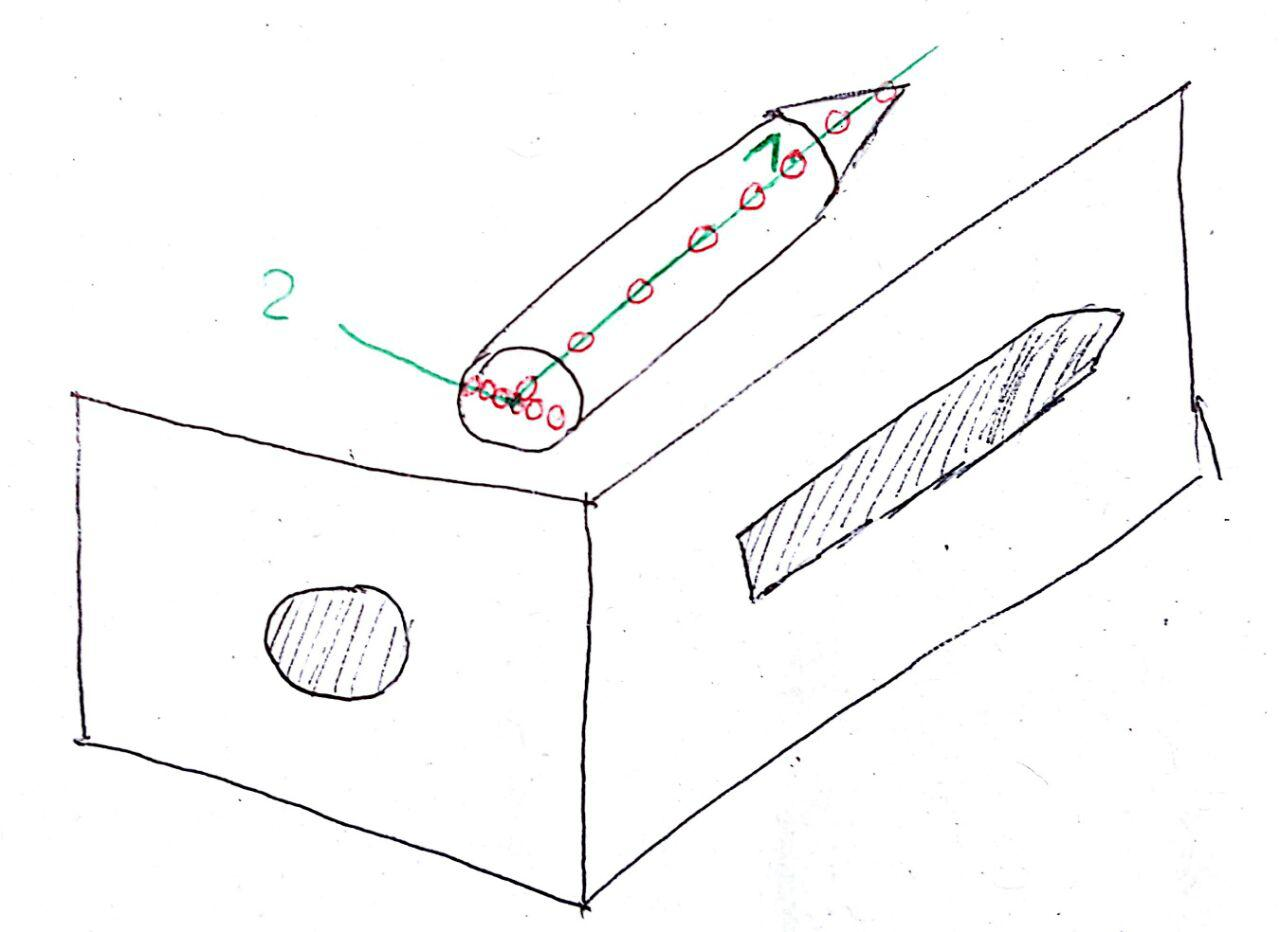
\includegraphics[width=0.5\linewidth]{llapis.jpg}
	\caption{Representació projecció llapis}
	\label{fig:llapis}
\end{figure}

Podem escollir diversos plans on projectar el llapis. Si es fa una projecció en alçat es veurà el llapis estirat i segons com es projecti de perfil només es veurà un cercle.

Quina de les dues representacions és millor? Què volem? 
\begin{itemize}
	\item Representar les dades de la manera més fidel? (Representació en alçat)
	\item Representar les dades de la manera més reduïda possible? (Representació de perfil)
\end{itemize}

També es poden representar les dades sobre l'eix de revolució del llapis. O sobre un eix perpendicular a aquest. El que busquem és que les dades tinguin la màxima variabilitat possible.

\textbf{Formalització}: Tenim una mostra de dades $\{x_1, ..., x_n\}$ tal que $x_i \in \mathbb{R}^d$; provenen d'un vector aleatori $X = (X_1, ..., X_d)^T$ que té mitjana $\mu \in \mathbb{R}^d$ i una matriu de covariàncies $\Sigma = \left\{ \sigma_{ij}^2 \right\}$.

\begin{itemize}
	\item $\mu = \mathbb{E}(X) = \mathbb{E}(X_1, ..., X_d)$
	\item $\Sigma = \mathbb{E}\left((X - \mu)(X-\mu)^T\right)$
	
	\begin{flalign*}
	\text{En particular } & CoVar(X_i, X_j) = \sigma_{ij}^2  &\\
 & CoVar(X_i, X_i) = \sigma_{ii}^2 = Var(X_i) =\sigma_i^2 &
	\end{flalign*}
\end{itemize}

Considerem el problema de trobar unes variables noves $Y = (Y_1, ..., Y_d)^T$ tal que:

\begin{enumerate}
	\item $CoVar(Y_i, Y_j) = 0$ per $i \ne j$
	\item $Var(Y_1) > Var(Y_2) > ... > Var(Y_d)$
	\item $\sum_{i=1}^d Var(X_i) = \sum_{i=1}^d Var(Y_i)$
\end{enumerate}

Busquem un \textbf{mètode lineal}: les $Y_j = a_j^TX, j=1,...,d$

Imposem una condició de \textbf{normalització} $||a_j||^2 = 1$ 
(Transformació \textbf{ortogonal})

\subsection{Tria de $a_1$}
Cal que $a_1$ maximitzi la $Var(Y_1)$ subjecte a $||a_1||^2=1$
$$ Var(Y_1) = Var(a_1^TX) = a_1^TVar(X)a_1 = a_1^T\Sigma a_1 $$

\textbf{Excursió}: multiplicadors de Lagrange

Sigui $f:\mathbb{R}^d \rightarrow \mathbb{R}$ diferenciable i la volem maximitzar subjecte a una \textbf{condició d'igualtat} $g(x_1, ..., x_d) = c$.

Una manera de fer-ho és construir el Lagrangià:

$$  L(x) = f(x) - \lambda(g(x) - c)  $$

La solució és un punt estacionari (les derivades s'anu\lgem en).
$$  \frac{\partial L}{\partial x_i} - \lambda \frac{\partial g}{\partial x_i} = 0, i = 1, ..., d \implies L(a_1) = a_1^T\Sigma a_1 - \lambda(||a||^2 - 1)  $$

\begin{itemize}
	\item $\frac{\partial L}{\partial a_1} = 2\Sigma a_1 - 2\lambda a1 = 0$
	\item $\Sigma a_1 = \lambda a_1$
	
	$a_1$ és un vector propi de $\Sigma$ amb valor propi $\lambda$
	\item $Var(Y_1) = a_1^T\Sigma a_1=a_1^T(\lambda a_1) = \lambda(a_1^T a_1) = \lambda ||a_1||^2 = \lambda$
	
	\textbf{Mètode}: triem $\lambda$ on el VAP $\Sigma$ més gran
	
	$\lambda_1, ..., \lambda_d \implies \lambda_1 > \lambda_2 > ... > \lambda_d > 0$
\end{itemize}

\subsection{Tria de $a_2$}

$Y_2 = a_2^TX$ on $||a_2||^2 = 1$ i $$ CoVar(Y_2, Y_1) = CoVar(a_2^TX, a_1^TX) = a_2^T\Sigma a_1 \underbrace{= 0}_\text{Volem que sigui 0} $$ 

$$  = a_2^T(\Sigma a_1) = a_2^T(\lambda_1 a_1) = \lambda_1 (a_2^Ta_1) \underbrace{= 0}_\text{volem que ho sigui} \Leftrightarrow a_1 \bot a_2  $$

$$  L(a_2) = a_2^T\Sigma a_2 - \lambda(||a_2||^2 - 1) - \delta(a_2^Ta_1) \implies \Sigma a_2 = \lambda a_2  $$

Triem $a_2$ com el vector associat al segon VAP més gran de $\Sigma \rightarrow \lambda_2$

\subsection{Resultats}
\begin{enumerate}
	\item Si diem $\Delta$ a la matriu de covariàncies de $Y$, és clar que
	\[ \Delta = 
	\begin{pmatrix}
	\lambda_1 &   &   & \text{\huge0 } \\
 & \lambda_2 &   &  \\
 &  & \ddots &  \\
 \text{ \huge0} &  &  &  \lambda_d
	\end{pmatrix} \]
	
	donats: $a_3, ..., a_d$ es deriven igual els $a_1, ..., a_d$ i es diuen \textbf{components principals}.
	
	\item Per construcció
	\begin{flalign*}			
		& \overset{Var(Y_1)\ >}{\underset{\lambda_1}{\verteq}} \overset{Var(Y_2)\ >}{\underset{\lambda_2}{\verteq}}
		\overset{...\ >\ Var(Y_d)}{\underset{\lambda_d}{\verteq}} &
	\end{flalign*}
 
	
	\item $\sum_{i=1}^d Var(Y_i) = \sum_{i=1}^d \lambda_i \underbrace{=}_\text{teorema} Tr(\Sigma) = \sum_{i=1}^d \sigma_i^2 = \sum_{i=1}^d Var(X_i)$
\end{enumerate}

\textbf{Idea}: quedar-se amb els $k$ primers components principals $a_1, ..., a_k\ (k<d)$ (Per visualitzar $k=\{2,3\})$. Si decidim quedar-nos amb les $k$ primeres:

$$ \%\text{de variància retinguda } = \frac{\sum_{i=1}^k \lambda(i)}{\sum_{i=1}^d \lambda(i)}·100 $$

% Formula 1 aquí

\textbf{Algorisme} PCA $(X, k = 2)$

\begin{itemize}
	\item Calcular la mitjana de les dades $\hat{\mu}$
	\item Centrar les dades $x_n \leftarrow x_n - \hat{\mu}, n = 1, ..., N$
	\item Calcular els VEPs i VAPs de $\hat{\Sigma}$
	
	ret $A \leftarrow (a_1, a_2, ..., a_k)$
\end{itemize}

\section{Anàlisi discriminant de Fisher}
$$  \mathcal{D} = \{(x_1, t_1), ..., (x_N, t_N)\}, \underline{\boldsymbol{x_n \in \mathbb{R}^d}}, t_n \in \{-1, +1 \}  $$

% Figura 2

\textbf{Notació}
$$  C_+, C_-  $$
\begin{align*}
	C_+ &:= \{ n | t_n = +1 \} \\
	C_- &:= \{ n | t_n = -1 \} \\
	\vec{m}_+ &:= \frac{1}{|C_+|} \sum_{n\in C_+} \vec{x}_n \\
	\vec{m}_- &:= \frac{1}{|C_-|} \sum_{n\in C_-} \vec{x}_n \\
\end{align*}

Si suposem que tenim un vector $D$-dimensional i el volem projectar a una dimensió estem buscant un $w$ tal que $y_n = w^T \vec{x}_n$. Així doncs, busquem un $w$ tal que maximitzi la separació entre les mitjanes projectades $m_+ - m_- = \vec{w}^T(\vec{m}_+ - \vec{m}_-)$ on $m_k = w^T \vec{m}_k$.

La \textbf{dispersió} (\emph{scatter}) d'una classe projectada:

$$  
s_+^2 := \sum_{n \in C_+} (y_n - m_+)^2 = 
\sum_{m \in C_+} (\vec{w}^T \vec{x}_n - \vec{w}^T \vec{m}_+)^2
$$
(és la variància, excepte la divisió per $|c_+| - 1$)

$s_-^2$ anàlogament 

$$
s_-^2 := \sum_{n \in C_-} (y_n - m_-)^2 = 
\sum_{m \in C_-} (\vec{w}^T \vec{x}_n - \vec{w}^T \vec{m}_-)^2
$$

La \textbf{dispersió total} és $s_+^2 + s_-^2$.

El criteri de Fisher és $$  J(\vec{w}) = \underbrace{\frac{|\vec{w}^T(\vec{m}_+-\vec{m}_-)|}{s_+^2 + s_-^2}}_\text{a maximitzar}  $$

La solució és $\vec{w}^* = S_w^{-1}(\vec{m}_- - \vec{m}_+)$

$S_w$ és la matriu de dispersió intra-classe (\emph{within-class scatter matrix}):

$$
S_w = S_+ + S_- = 
\underbrace{\sum_{n \in C_+} (x_n - \vec{m}_+)(x_n - \vec{m}_+)^T}_{S_+} +
\underbrace{\sum_{n \in C_-} (x_n - \vec{m}_-)(x_n - \vec{m}_-)^T}_{S_-}  
$$


$S_B$ és la matriu de dispersió inter-classe (\emph{between-class scatter matrix}):
$$
S_B = (\vec{m}_2 - \vec{m}_1)(\vec{m}_2 - \vec{m}_1)^T
$$

	
\end{document}